\chapter{}
\section{Per-event Log-likelihood Ratio}
\label{app:pereventllr}
The combined observed significance from the ICHEP 2012 dataset, corresponding to $4.9\sigma$, 
is driven largely by the two high resolution channels $\Hgg$ and $\Hzzl$. Those two channels
alone combine provide a significance of $5.0\sigma$ at $\mh=125$ GeV. 
Before entering the likelihood of Equation~\ref{eqn:likelihood}, the contribution from the 
events in each channel are first combined. For each channel, the sum over events $i$,
\begin{equation}
\log \call_{\mathrm{channel}}(\mathrm{data}|\mu) = \sum_{i}\log\call(i|\mu),
\end{equation}
represents summing the per-event log-likelihood at a given value of $\mu$. As usual, the 
value of $\mh$ is implicitly assumed in the definition of the likelihood, $\call$.
Here the nuisance parameters are not explicitly indicated, although they are profiled in the usual way at a given value of $\mu$.
The test-statistic appropriate for 
determining significances, $q_{0}$, can be expressed as the difference in the negative 
log-likelihoods ($\Delta(nll)$) for $\mu=0$ and $\mu=\hat{\mu}$ (the best fit signal strength),
\begin{equation}
q_{0} = -2\left[\log\call(i|\mu=\muhat) - \log\call(i|\mu=0) \right]= 2\Delta(nll).
\end{equation}

The individual contribution from each event in data in each channel can therefore be determined
by considering the per-event delta log-likelihood. Figure~\ref{fig:perevllr} shows the distribution
of the per-event log-likelihood in data for the $\Hgg$ and $\Hzz$ channels.
The distributions expected under the background-only and signal-plus-background hypotheses, where 
$\mu$ is set to the best fit value, are also shown. 
In these two channels, there is an additional term in the likelihood which 
represents the normalization of the signal plus background model as the likelihood 
in these cases is unbinned. It should be noted that the 
best fit value for $\mu$ is evaluated from the combined data in the $\Hgg$ and $\Hzz$ 
channels so that the individual contributions from each datum can be positive or negative.


\begin{figure}
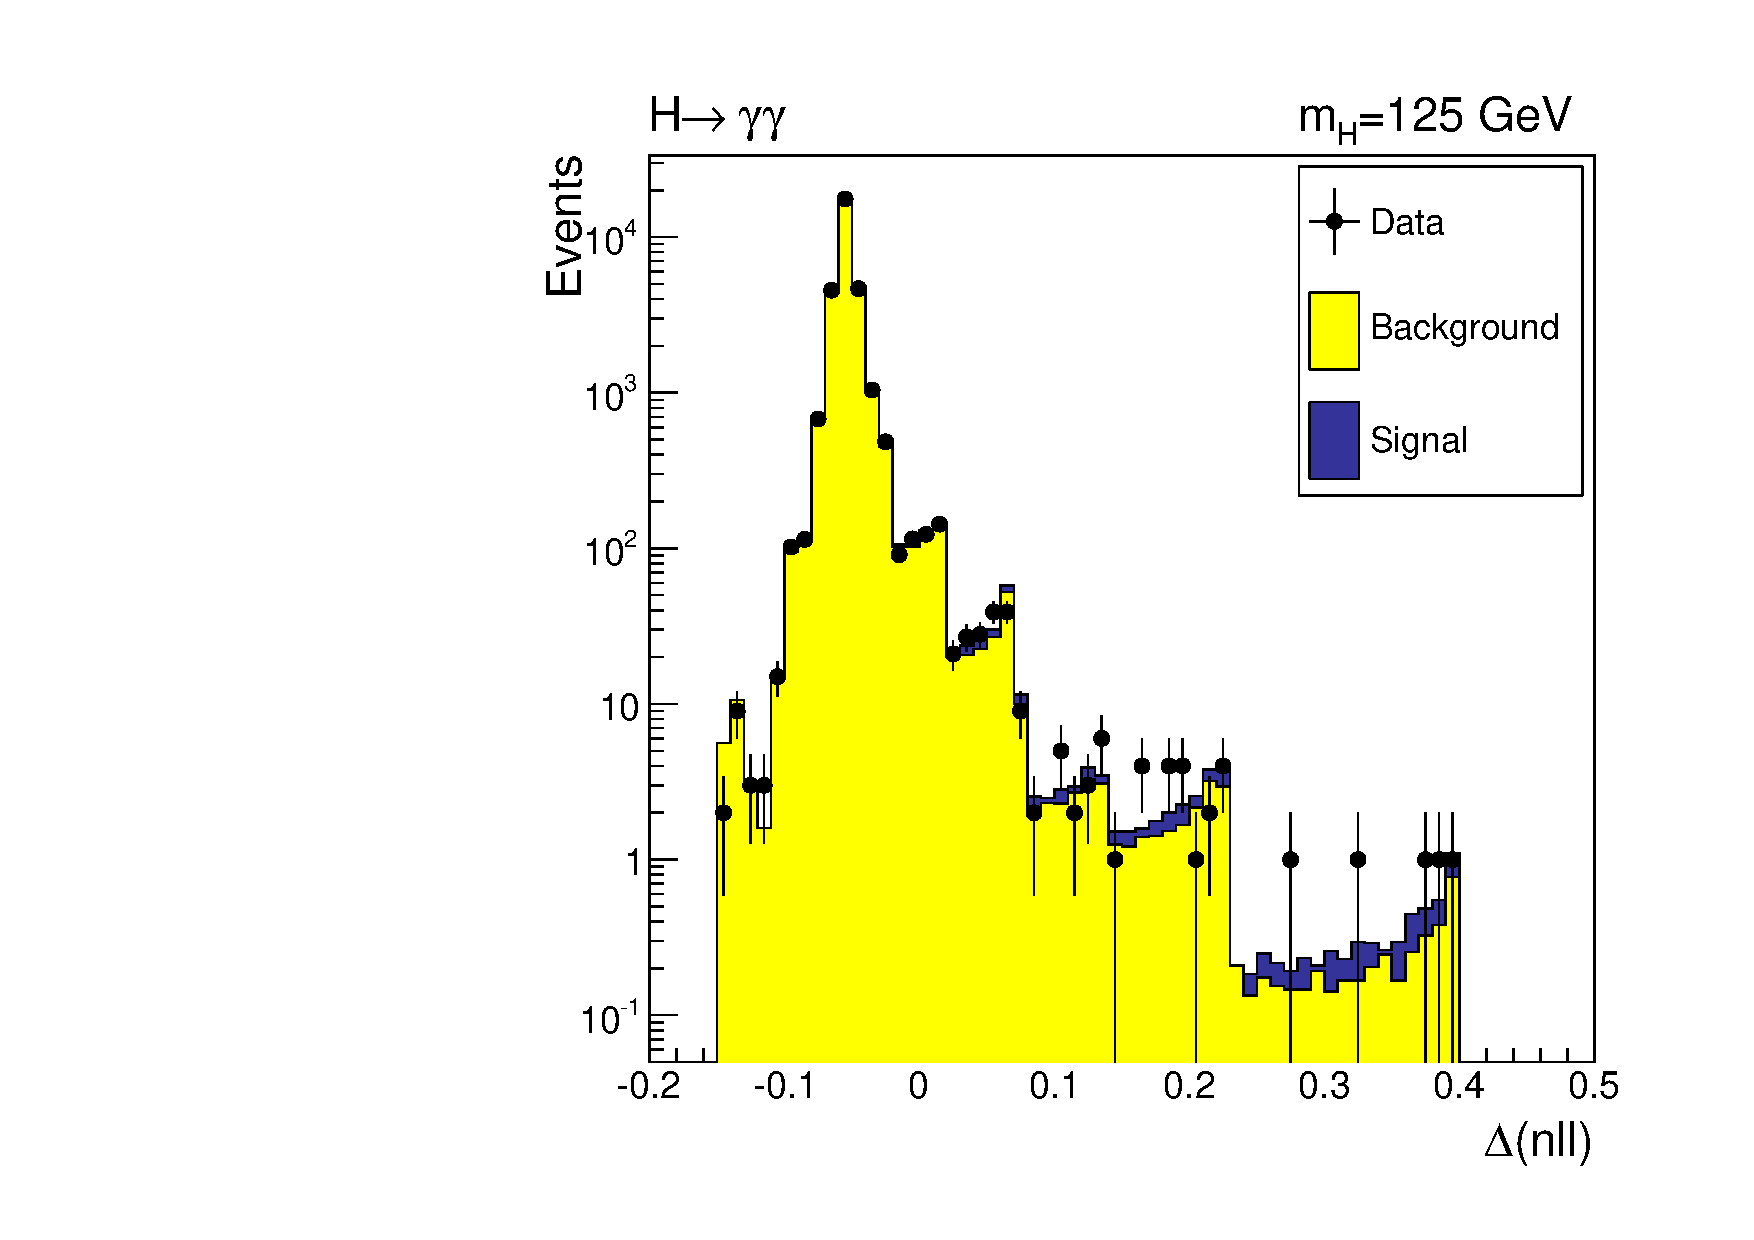
\includegraphics[width=0.49\textwidth]{combinations/perEvLLR_hgg8TeV.pdf}
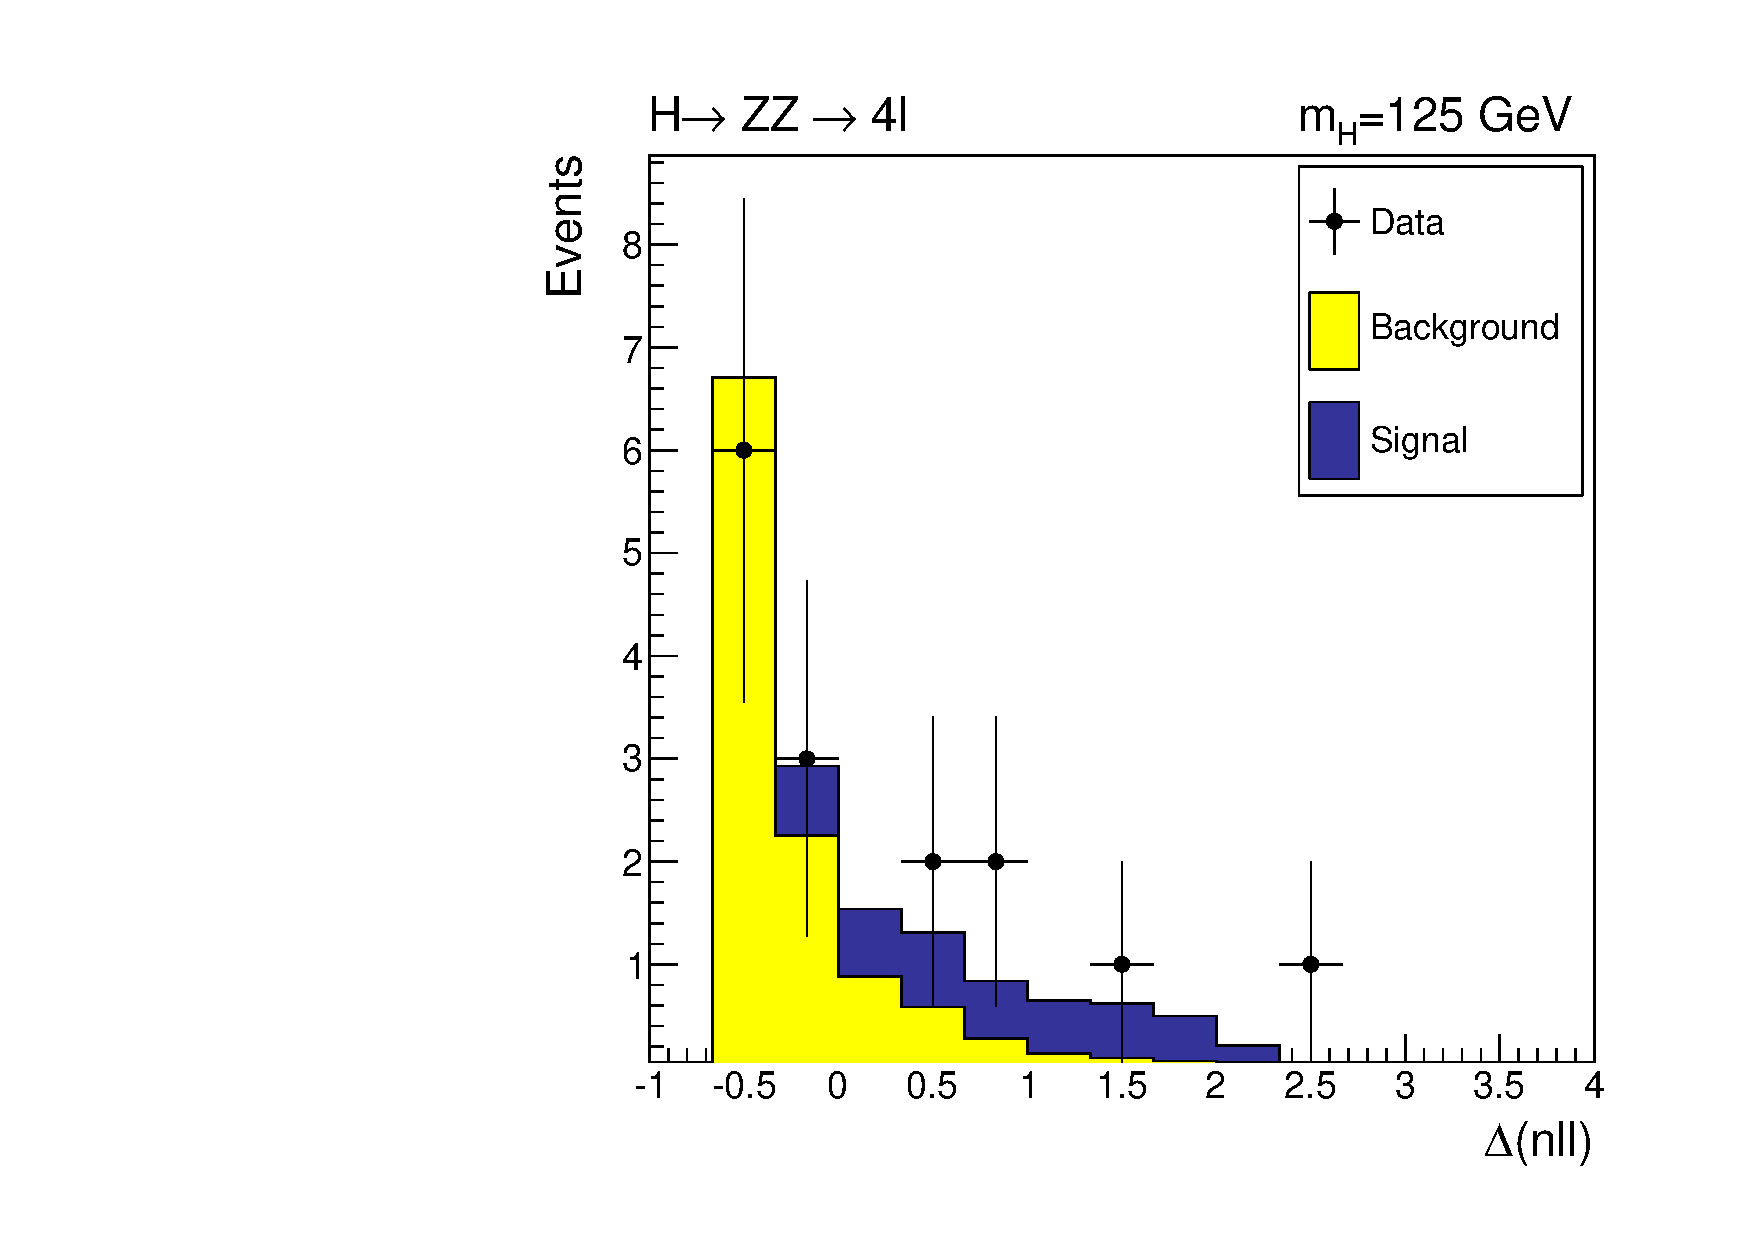
\includegraphics[width=0.49\textwidth]{combinations/perEvLLR_hZZ4l.pdf}
\caption{Per-event delta negative log-likelihood ($\Delta nll$) distributions for the 
background-only and signal-plus-background hypotheses in the ICHEP 2012 $\Hgg$ (left) and $\Hzzl$ (right)
analyses. The distributions for the observed events from each channel are indicated by the black points.
The likelihoods are evaluated for $\mh=125$ GeV at the best fit values of $\mu$ from the combination 
of these two channels only.}
\label{fig:perevllr}
\end{figure}



\section{Feldman-Cousins Boundary Effects}
\label{app:fcboundaryeffects}
The Feldman-Cousins procedure used to check the compatibility of the new observed
particle with the Standard Model Higgs boson typically produces the same 68\% confidence
contours as obtained from scanning $q_\boldmu$. 
Disagreement between the two methods is usually observed where the best fit value
is outside the physically allowed region. However, for contours which are close to the
boundaries of the physical region, the two methods will yield different results even
if the best fit point is inside the allowed region.
A simple demonstration of this effect can be seen in Figure~\ref{fig:comparefclh}
which shows two contours in the $\muqqh,~\muggh$ plane obtained from data
in the $\Hgg$  analysis on the ICHEP dataset. The signal extraction technique 
used here is the binned technique described in Section~\ref{sec:signalextraction}.
The two contours shown are those at the 50\% and 75\% confidence levels from each
method. These contours are chosen specifically in this case to demonstrate the effect
of the boundaries at $\muqqh=0$ and $\muggh=0$. Although the 50\% contours
agree well between the two methods, disagreement can be seen between the 75\% contours
where the contour is close to one of the boundaries.

\begin{figure}
\begin{center}
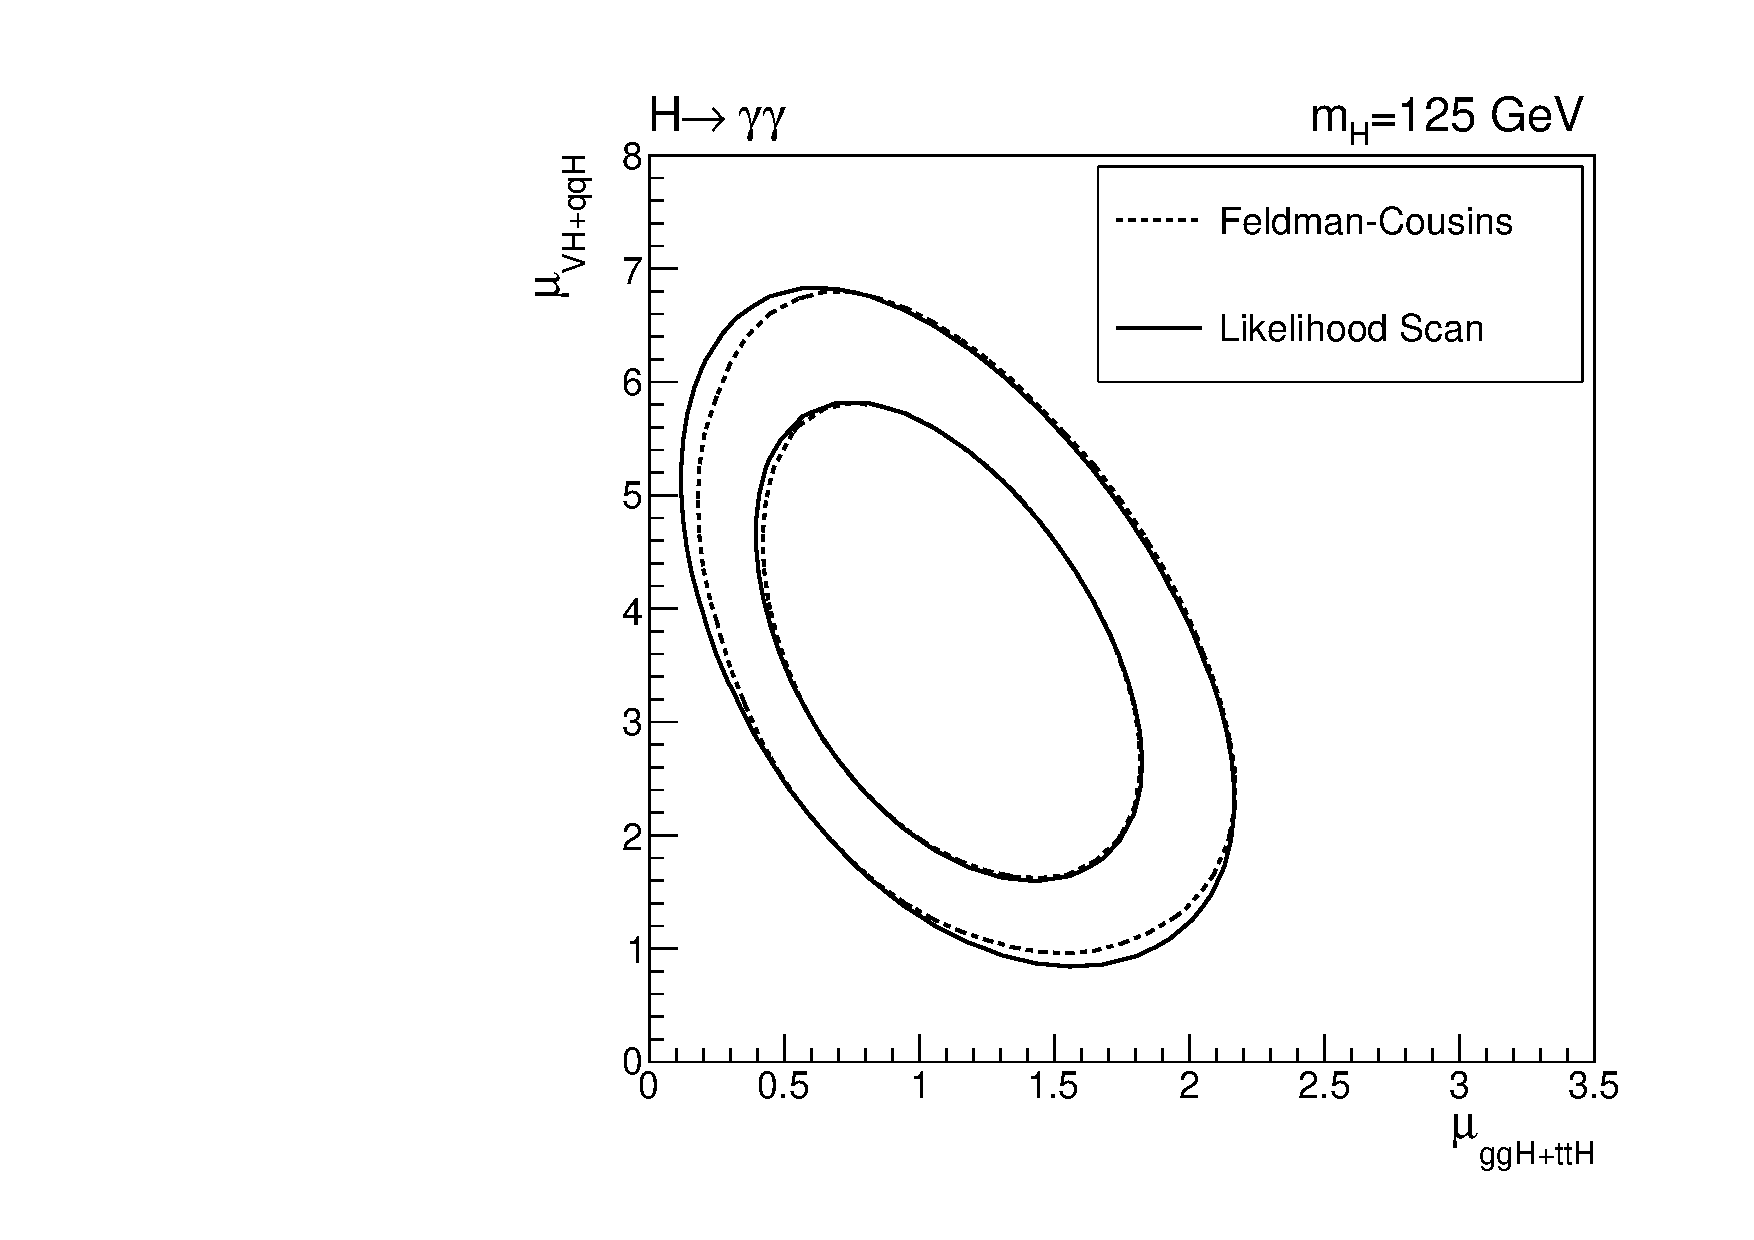
\includegraphics[width=0.8\textwidth]{combinations/compare-fc-lh.pdf}
\end{center}
\caption{Comparison between 50\% (inner) and 75\% (outer) contours in data from the $\Hgg$ 
channel as determined using the Feldman-Cousins and a scan of $q_{\boldmu}$ (labelled ``Likelihood Scan'').
In the Feldman-Cousins technique, the constraints, $\muggh \ge 0$ and $\muqqh \ge 0$ are 
imposed. }
\label{fig:comparefclh}
\end{figure}
